Soit $ABC$ un triangle aigu tel que $AB<AC$. Soient $E$ et $F$ les pieds des hauteurs issues de $B$ et $C$, respectivement, et soit $M$ le milieu de $BC$. La droite tangente au cercle circonscrit à $ABC$ en $A$ coupe la droite $BC$ en $P$. La droite passant par $A$ parallèle à la droite $BC$ coupe la droite $EF$ en $Q$. Montrer que la droite $PQ$ est perpendiculaire à la droite $AM$.

\textbf{Première solution:} (Patrick, by Arnaud)

Comme dans la deuxième preuve, on obtient $\angle QAE=\angle AFE$ et donc $C$ se trouve sur la tangente an $A$ au cercle circonscrit au triangle $AFE$. En particulier, $QA^2=QE\cdot QF$. De même, $PA^2=PB\cdot PC$. Enfin, on remarque que les points $BCEF$ se trouvent sur un cercle.

L'astuce est maintenant de considérer le point $A$ comme un cercle dégénéré d'un seul point. La puissance de $P$ par rapport à ce point et $PA^2$ et celle de $Q$ est $QA^2$. Comme $PA^2=PB\cdot PC$ et $QA^2=QE\cdot QF$, les points $P$ et $Q$ se trouvent sur la ligne de puissance des cercles $BCEF$ et $A$. En particulier $PQ$ est perpendiculaire à la droite passant par $A$ et le centre du cercle $BCEF$ qui est précisément le point $M$.

\textbf{Deuxième solution:} (Arnaud)

On tente une approche vectorielle (motivée par la donnée de $M$ en tant que milieu et l'orthogonalité désirée). Sans passer par des coordonnées, on doit montrer que 
\[
\vec{AM}\cdot \vec{PQ}=0.
\]
Observer que $\vec{PQ}=\vec{PA}+\vec{AQ}$ et, comme $M$ est le milieu de $BC$, $2\vec{AM}=\vec{AB}+\vec{AC}$. Il suffit donc de montrer que 
\[
(\vec{PA}+\vec{AQ})\cdot(\vec{AB}+\vec{AC})=0\Leftrightarrow \vec {AQ}\cdot \vec{AB}+\vec{AQ}\cdot\vec{AC}=\vec{AP}\cdot \vec{AB}+\vec{AP}\cdot\vec{AC}.
\]
La stratégie est de calculer chacun des quatre produits que l'on obtient en développant le membre de gauche à l'aide de la formule $\vec v\cdot \vec w=|v|\cdot|w|\cdot \cos(\theta)$ (et donc sans passé par des coordonnées !). Il faut donc trouver des relations entre les longueurs $|AP|,|AB|,|AC|,|AQ|$ et les angles entre ces segments.

Un peu de chasse aux angles nous donne: $\angle PAB=\angle ACB=\gamma$ en utilisant les propriétés des tangentes, $\angle QAC=\gamma$ par parallélisme, $\angle AFQ=\gamma$ en utilisant que $FEBC$ est inscrit. De même, $\angle AEF=\angle ABC=\beta$. En contemplant la figure, on remarque alors que $\Delta QAE\sim \Delta PBA$, car les deux triangles ont les mêmes angles. On en déduit
\[
\frac{|AQ|}{|AP|}=\frac{|AE|}{|AB|}
=\cos(\alpha).
\]
La dernière égalité est une application de la trigonométrie dans le triangle $AEB$ rectangle en $E$. Par le théorème du sinus, dans le triangle $ABC$, on obtient 
\[
\frac{|AB|}{|AC|}=\frac{\sin(\gamma)}{\sin(\beta)}.
\]

La relation de vecteurs désirée devient, en utilisant $\cos(\alpha+\gamma)=\cos(\pi-\beta)=-\cos(\beta)$, 
\begin{align*}
\vec {AQ}\cdot \vec{AB}+\vec{AQ}\cdot\vec{AC}&=\vec{AP}\cdot \vec{AB}+\vec{AP}\cdot\vec{AC}\\
\Leftrightarrow\frac{|AQ|}{|AP|}\left(\frac{|AB|}{|AC|}\cos(\alpha+\gamma)+\cos(\gamma)\right)&=\left(\frac{|AB|}{|AC|}\cos(\gamma)+\cos(\alpha+\gamma)\right)\\
\Leftrightarrow \cos(\alpha)\left(\frac{-\sin(\gamma)\cos(\beta)}{\sin(\beta)}+\cos(\gamma)\right)&=\frac{\sin(\gamma)\cos(\gamma)}{\sin(\beta)}-\cos(\beta)\\
\Leftrightarrow \cos(\alpha)(\sin(\beta)\cos(\gamma)-\sin(\gamma)\cos(\beta))&=\sin(\gamma)\cos(\gamma)-\sin(\beta)\cos(\beta)\\
\Leftrightarrow \cos(\alpha)\sin(\beta-\gamma)&=1/2(\sin(2\gamma)-\sin(2\beta))\\
\Leftrightarrow \cos(\alpha)\sin(\beta-\gamma)&=\cos(\beta+\gamma)\sin(\gamma-\beta)\\
\Leftrightarrow -\cos(\alpha)&=\cos(\beta+\gamma).
\end{align*}

La dernière égalité est vérifiée, car, de nouveau, $\cos(\beta+\gamma)=\cos(\pi-\alpha)=-\cos(\alpha)$. On a utilisé plusieurs identités trigonométriques comme la formule pour le sinus d'une différence, l'imparité du sinus, le sinus du double d'un angle ou encore la formule par exprimer une différence de deux sinus comme un produit.

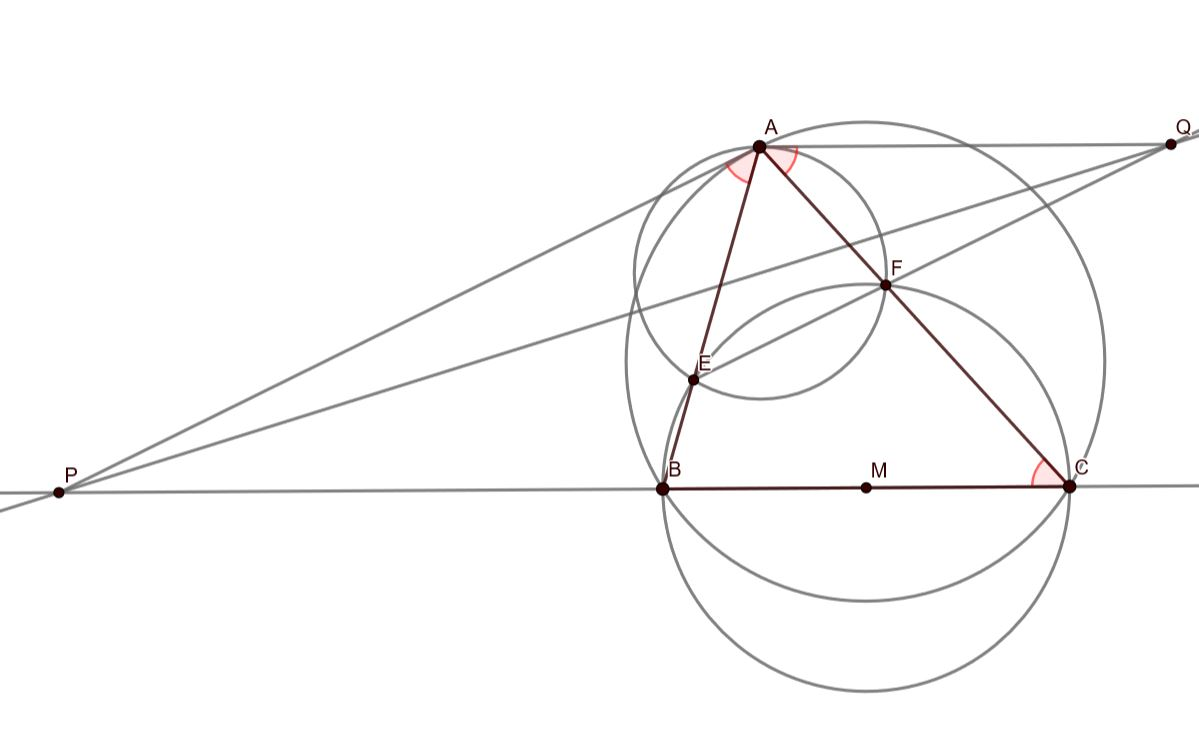
\includegraphics[width = 0.8\textwidth]{solutions/s9_picture.JPG}

\newpage
\textbf{Marking Scheme:}

\begin{itemize}
    \item First solution:

\begin{itemize}
    \item 0P: $PA^2=PB\cdot PC$ or $BCEF$ lie on a circle
    \item 1P: basic angle chasing that leads to one relation of type: $QA^2=QE\cdot QF$.
      \item 2P: reformulating the conclusion in terms of power lines by observing that $M$ is the center of $BCEF$ and that 
    \item 4P: Conclusion
\end{itemize}
  
    \item Second solution
    
    \begin{itemize}
    \item 1P: basic angle chasing that leads to the relation that one of the triangle $\Delta PBA$ or  $\Delta PAC$ is similair to one of the triangle $\Delta QEA$ or $\Delta QAF$ or equivalently proving that two angles are the same
    \item 2P: reformulating the conclusion with a vector relation where one used that $M$ is the midpoint of $BC$
    \item 4P: conclusion
\end{itemize}

\end{itemize}